\documentclass[11pt,a4paper]{article}

% --- Layout
\usepackage[a4paper,margin=2.4cm]{geometry}
\usepackage{microtype}
\usepackage{parskip}

% --- Math
\usepackage{amsmath,amssymb,amsthm}
\usepackage{mathtools}
\usepackage{bm}

% --- Graphics & tables
\usepackage{graphicx}
\usepackage{booktabs}
\usepackage{array}

% --- References
\usepackage[numbers,sort&compress]{natbib}
\bibliographystyle{plainnat}

% --- Hyperlinks (load last)
\usepackage[colorlinks=true,linkcolor=blue!50!black,citecolor=blue!50!black,urlcolor=blue!50!black]{hyperref}

% --- Macros
\newcommand{\F}{\lvert F\rvert}
\newcommand{\Gk}{\lvert G_k\rvert}
\newcommand{\Gkm}{\lvert G_{k-1}'\rvert}
\newcommand{\Gkmm}{\lvert G_{k-2}'\rvert}
\newcommand{\Gkp}{\lvert G_k'\rvert}

\title{An IIR-filter view of the Overdrive variant: multiplicative\\[2pt]
       momentum acceleration of the IFTA for kinoform synthesis}
\author{Marc Bernau\thanks{\texttt{bernau.marc@googlemail.com}}}
\date{Preprint, May 2026}

\begin{document}
\maketitle

\begin{abstract}
Accelerating the iterative Fourier transform algorithm (IFTA) for kinoform
synthesis with classical momentum on the phase, on the gradient of a
Wirtinger-flow loss, or on additive correction vectors generally fails: the
constraint sets are non-convex, the iterate lives on a torus, and
Euclidean momentum amplifies the wrong directions. The \emph{Overdrive}
update rule, introduced in 2007 as an ad-hoc accelerated GS variant, can
instead be read as Polyak's heavy-ball momentum applied to the
log-amplitude in the negative-entropy (Itakura--Saito) mirror geometry.
In this view it is, by direct construction, a first-order infinite impulse
response (IIR) filter with pole at $z=\beta$, and closing the loop through
the Gerchberg--Saxton (GS) projection produces a closed-loop pole at
$z=\beta-c$, where $c$ is the local contraction rate of GS. The iteration
is stable for every $\beta\in(0,1)$, with fastest transient decay at
$\beta\approx c$. Empirically, the innovation process driving the
closed-loop recursion is colored (lag-1 autocorrelation $\approx 0.9$);
the AR(1)-with-white-noise model that would predict a closed-form synthesis
floor is therefore informative only at the level of \emph{ranking} $\beta$
values, not as a quantitative predictor. The natural Lyapunov candidate is
the log-spectral distance (the Bregman divergence of the mirror map), not
the L\textsuperscript{2} hologram-plane error; this resolves the apparent
paradox that the hologram-plane correction vector grows transiently while
the image-plane error decreases. On 29 natural grayscale images, Overdrive
at $\beta=0.7$ reaches a mean PSNR of $32.4$~dB after twenty iterations,
which exceeds plain GS by $7.5$~dB, HIO/RAAR/WGS by at least $6.9$~dB,
phase-domain Polyak momentum by $8.6$~dB, and Nesterov-accelerated Wirtinger
Flow --- the natural additive-momentum competitor --- by $4.1$~dB. A
reference Python implementation is provided.
\end{abstract}

% =====================================================================
\section{Introduction}
% =====================================================================

Two superficially similar problems are routinely conflated in the literature.
\emph{Phase retrieval} starts from a known intensity that arose from some
unknown phase, and asks to recover that phase: the true solution exists by
construction. \emph{Kinoform synthesis} \cite{Lesem1969,Soifer1997} starts
from a desired grayscale intensity and asks to design a phase pattern,
modulating a uniform-amplitude wave, whose Fourier transform reproduces it.
For grayscale targets such an exact phase pattern generally does not exist:
the constraint sets in the two planes do not intersect, the problem is
nonconvex, many-to-one, and saturated with symmetries. Any iterative
algorithm therefore terminates not at a true solution but at a \emph{limit
cycle of alternating projections} whose distance to the target is the
irreducible synthesis floor.

This distinction matters for what one can hope to prove. The
Gerchberg--Saxton algorithm \cite{Gerchberg1972} and its many descendants
\cite{Fienup1978,Fienup1980,Prongue1992,Bengtsson1998,Liu2006} solve the
kinoform synthesis problem by alternating Fourier projections and remain the
workhorse of real-time hologram generation on phase-only spatial light
modulators. The Hybrid Input--Output algorithm \cite{Fienup1982} adds
input-plane feedback for phase retrieval and is the canonical extension of
GS in that setting; the Relaxed Averaged Alternating Reflections (RAAR)
algorithm \cite{Luke2005} replaces alternating projections with averaged
reflections for problems with two magnitude constraints; and the Weighted GS
algorithm \cite{DiLeonardo2007} adds a cumulative pixelwise weighting scheme
originally designed for spot-array generation. Section~\ref{sec:numerics}
benchmarks all three. Modern phase-retrieval methods --- Wirtinger Flow
\cite{Candes2014} and randomly-initialized gradient descent \cite{Chen2018}
--- give global convergence guarantees, but those guarantees apply to a
problem in which a true solution exists; they do not transfer to the kinoform
case, where no such solution does. Deep-learning approaches
\cite{Zheng2021,Sun2022,Zhu2025} and Camera-in-the-Loop training
\cite{Peng2020} sidestep iteration altogether at the cost of training data
and dedicated hardware. For real-time video projection on
commodity hardware --- our motivating application --- the classical
multiplicative IFTA family remains attractive: nearly as cheap as GS per
iteration, no training, convergence in about a dozen FFT cycles. The
question for these algorithms is therefore not ``do they reach the target?''
(no) but ``how close to the limit cycle do they settle, and how is the
synthesis floor controlled by the algorithm parameter?''.

\paragraph{Three families of acceleration.} The classical algorithms in
the previous paragraph split naturally into three families by where they
inject ``memory'' between iterations.
\begin{description}
  \item[Alternating projections (no momentum).] GS, HIO, RAAR, and
        weighted GS all proceed by two-plane projections; only their
        feedback rules and (in HIO) the input-output coupling differ.
  \item[Additive momentum (Euclidean).] Phase-domain Polyak momentum (here
        called MGS) updates the phase by
        $\phi_k = \phi_{k-1} + \Delta_k + \mu\,(\phi_{k-1}-\phi_{k-2})$,
        and Nesterov-accelerated Wirtinger Flow (NWF) does the same on
        the complex iterate after a Wirtinger gradient step. Both treat
        the iterate as living in a Euclidean space.
  \item[Multiplicative momentum (log-space).] The Fienup amplitude rule
        \cite{Fienup1978}, Bengtsson rule \cite{Bengtsson1998}, and
        Overdrive rule \cite{Bernau2007} re-impose the Fourier-plane
        amplitude constraint by mixing the target with the current and
        previous reconstructions through \emph{products} of amplitudes.
        After logarithms, the mixing becomes additive in log-amplitudes
        --- the natural mirror coordinate for non-negative quantities.
\end{description}
The contribution of this note is twofold. First, we show that the third
family --- specifically the Overdrive rule --- admits a clean IIR
interpretation (Section~\ref{sec:log}) and is equivalent to Polyak
momentum in the negative-entropy mirror geometry
(Section~\ref{sec:mirror}). Second, we benchmark all three families on a
common image set (Section~\ref{sec:numerics}) and find that the
multiplicative family dominates, with Overdrive at $\beta=0.7$ exceeding
the best additive-momentum competitor (NWF) by $4.1$~dB.

Among the multiplicative IFTA variants, the \emph{Overdrive} rule introduced
in \cite{Bernau2007} and analyzed empirically in \cite{Bernau2012}
\begin{equation}
  \Gkp \;=\; \Gkm^{\beta}\;\frac{\F^{\,2-\beta}}{\Gk}, \qquad \beta\in(0,1),
  \label{eq:overdrive}
\end{equation}
consistently yields the lowest synthesis floor of any multiplicative
variant we tested, but its stability and the size of that floor have so far
been demonstrated only by simulation. The dissertation
\cite[Sec.~4.4]{Bernau2012} states that stability ``cannot be shown
analytically from the geometric vector argument''. Two issues stand in the
way:
\begin{enumerate}
  \item In the hologram plane, the L\textsuperscript{2} norm of the correction
        vector is generally \emph{larger} than the previous error, so the
        usual GS-style monotonicity argument fails.
  \item The parameter $\beta$ enters the rule \emph{nonlinearly}, so the
        cosine-rule argument used by Fienup \cite{Fienup1980} does not apply.
\end{enumerate}

In this note we resolve both issues by working in log-amplitudes around the
algorithmic limit cycle, not around an idealized target solution.
Section~\ref{sec:rule} restates the Overdrive rule and its series expansion.
Section~\ref{sec:log} shows that taking logarithms turns the update into a
first-order linear difference equation, exposing an IIR-filter structure with
explicit pole at $z=\beta$. Section~\ref{sec:mirror} re-derives the same rule
as Polyak heavy-ball momentum in the negative-entropy mirror geometry,
making the connection to the broader momentum-method literature explicit.
Section~\ref{sec:stability} linearizes the closed iteration around the limit
cycle and gives the pole-based stability condition and the locally optimal
$\beta$. Section~\ref{sec:lyapunov} identifies the log-spectral distance ---
the Bregman divergence of the mirror map --- as the right Lyapunov
candidate; Section~\ref{sec:stochastic} discusses the steady-state synthesis
floor as a function of $\beta$, and reports an empirical test showing that
the AR(1)-with-white-noise closed-loop model is qualitatively but not
quantitatively correct. Section~\ref{sec:numerics} benchmarks the algorithm
against representatives of all three families on a $29$-image natural
grayscale test set.

% =====================================================================
\section{The Overdrive rule}\label{sec:rule}
% =====================================================================

We adopt the notation of \cite{Bernau2012}. Let $F\in\mathbb{C}^{H\times W}$ be
the desired complex amplitude in the image plane, $\theta_k$ the hologram
phase at iteration $k$, and $G_k=\mathcal{F}\{u\,e^{j\theta_k}\}$ the current
reconstruction, where $u$ is the (uniform) laser amplitude and $\mathcal{F}$
the discrete Fourier transform. The Overdrive rule \eqref{eq:overdrive}
re-imposes the Fourier-plane amplitude constraint by mixing the previous
\emph{virtual} amplitude $\Gkm$ with the target $\F$, modulated by the inverse
of the current reconstruction $\Gk$. The exponents $\beta$ and $2-\beta$ are
chosen so the total exponent on the right-hand side equals one; this
dimensional balance is what makes the log-domain analysis below possible.

After a few warm-up iterations of plain GS (so that $\Gkm\approx\F$), the
recursion can be unrolled. Setting $\Gkm = \F$ for $k\le k_0$ and substituting
into \eqref{eq:overdrive} gives, after $N$ Overdrive steps starting at
$k=k_0$,
\begin{equation}
  \Gkp_N \;=\; \F\;\prod_{k=0}^{N}
            \frac{\F^{\,\beta^{k}}}{\Gk^{\,\beta^{N-k}}}
        \;=\; \F\cdot\frac{\F}{\Gk_N}\,
                  \biggl(\frac{\F}{\Gk_{N-1}}\biggr)^{\!\beta}\!\cdot\ldots
                  \cdot\biggl(\frac{\F}{\Gk_0}\biggr)^{\!\beta^N}\!\!\!,
  \label{eq:product}
\end{equation}
where the index has been re-zeroed to $k_0$. The product structure reveals
the algorithm's intent: each new virtual amplitude is the target $\F$ times a
geometric-weighted product of past correction ratios $\F/\Gk_k$, with the most
recent correction weighted unity and older corrections weighted $\beta,
\beta^2,\ldots$.

A subtle but important property of \eqref{eq:product} is the symmetry of the
exponents. \emph{If} a configuration $\Gk=\F$ for all~$k$ were attainable,
the numerator and denominator exponents would sum to the same value,
$\sum_{k=0}^{N}\beta^{k}=\sum_{k=0}^{N}\beta^{N-k}$, the product would equal
one, and we would have $\Gkp_N=\F$ --- so an exact target would be a fixed
point of the rule. The dimensional balance is what guarantees this property;
the exponent $2-\beta$ in \eqref{eq:overdrive} was chosen for exactly this
reason.

In a real kinoform problem no such configuration exists: the alternating
projections do not produce $\Gk=\F$ but instead settle at a non-zero limit
$\Gk\to\Gk_{\!\infty}\neq\F$. We retain the term ``fixed point'' below in
the dynamical-systems sense (the limit point of the iteration map), with
the understanding that this point lies at a positive distance from $\F$.

% =====================================================================
\section{Log-domain analysis}\label{sec:log}
% =====================================================================

Define the log-amplitude residuals
\begin{equation}
  u_k \;:=\; \ln\frac{\Gkp}{\F}, \qquad
  v_k \;:=\; \ln\frac{\Gk}{\F}.
\end{equation}
Taking logarithms of both sides of \eqref{eq:overdrive} yields
\begin{equation}
  \boxed{\;u_k \;=\; \beta\,u_{k-1} - v_k.\;}
  \label{eq:iir}
\end{equation}
This is a first-order linear difference equation: a one-pole IIR filter
applied to $-v_k$, with pole at $z=\beta$ and DC gain $-1/(1-\beta)$. Stability
of the filter alone --- ignoring the closed loop, treating $v_k$ as exogenous
input --- requires $\lvert\beta\rvert<1$, the standard pole-radius condition.

The explicit solution to \eqref{eq:iir} with $u_{-1}=0$ is
\begin{equation}
  u_N \;=\; -\!\sum_{k=0}^{N}\beta^{N-k}\,v_k,
  \label{eq:explicit}
\end{equation}
which is exactly \eqref{eq:product} after taking logarithms. The mixing
parameter $\beta$ is therefore precisely the \emph{memory time constant} of an
exponentially-weighted moving average of past log-errors, with effective time
constant $\tau = -1/\ln\beta$. The values $\beta=0.5$ and $\beta=0.9$
correspond to $\tau\approx 1.4$ and $\tau\approx 9.5$ iterations, respectively.

This recovers the qualitative ``low-pass over the iteration history''
description of \cite{Bernau2012} as a quantitative statement: the Overdrive
rule is the \emph{exponential moving average of the log-error} re-applied as a
correction to the next virtual amplitude.

% =====================================================================
\section{Mirror-descent interpretation}\label{sec:mirror}
% =====================================================================

The IIR view of Section~\ref{sec:log} is signal-processing flavor. We now
give a second, optimization-flavor derivation that arrives at the same
update rule starting from Polyak's heavy-ball method, and explains
\emph{why} log-amplitudes are the natural coordinates: they are the mirror
coordinates of the negative-entropy potential on the positive orthant.

\paragraph{Polyak momentum in the Euclidean setting.} For minimizing a
smooth $f(x)$ on $\mathbb{R}^n$, Polyak's heavy ball is
\begin{equation}
  x_{k+1} \;=\; x_k - \alpha\,\nabla f(x_k) + \mu\,(x_k - x_{k-1}),
\end{equation}
with momentum coefficient $\mu\in[0,1)$. Its $Z$-transfer function from
$-\alpha\nabla f$ to $x$ is a one-pole IIR filter with pole at $z=\mu$. For
the kinoform problem the natural variable is a vector of non-negative
amplitudes, which lives on the positive orthant rather than in
$\mathbb{R}^n$; vanilla Euclidean heavy-ball both leaves the orthant and
amplifies the wrong directions in the non-convex constraint geometry. The
phase-domain heavy-ball variant of Section~\ref{sec:numerics} (MGS)
confirms this empirically: even at small $\mu$ it underperforms plain GS.

\paragraph{Mirror descent.} Mirror descent \cite{Beck2003,Bubeck2015}
replaces the Euclidean inner product with a strictly convex
``potential'' $\psi(x)$, performing the gradient step in the
\emph{mirror} coordinate $y=\nabla\psi(x)$ rather than in $x$ itself:
\begin{equation}
  \nabla\psi(x_{k+1}) \;=\; \nabla\psi(x_k) - \alpha\,\nabla f(x_k).
\end{equation}
For non-negative variables on the positive orthant the canonical choice
is the negative entropy
\begin{equation}
  \psi(x) \;=\; \sum_i x_i \ln x_i - x_i,
  \qquad
  \nabla\psi(x) \;=\; \ln x.
\end{equation}
Mirror descent under this potential becomes the multiplicative update
$x_{k+1} = x_k\,e^{-\alpha\nabla f(x_k)}$, the entropic mirror descent of
\cite{Beck2003}.

\paragraph{Heavy-ball mirror descent gives Overdrive.} Adding Polyak
momentum in the mirror coordinate gives
\begin{equation}
  \nabla\psi(x_{k+1}) \;=\; \nabla\psi(x_k) - \alpha\nabla f(x_k)
                          + \mu\bigl(\nabla\psi(x_k) - \nabla\psi(x_{k-1})\bigr).
\end{equation}
Specializing to $\psi=$ negative entropy and rewriting in
$x$-coordinates,
\begin{equation}
  \ln x_{k+1} \;=\; (1+\mu)\ln x_k - \mu\ln x_{k-1} - \alpha\nabla f(x_k),
\end{equation}
or equivalently
\begin{equation}
  x_{k+1} \;=\; \frac{x_k^{\,1+\mu}}{x_{k-1}^{\,\mu}}\,e^{-\alpha\nabla f(x_k)}.
  \label{eq:mirror-heavy-ball}
\end{equation}
For the kinoform problem the role of $x$ is played by the virtual
amplitude $|G_{k-1}'|$, the role of the gradient step
$e^{-\alpha\nabla f}$ is played by the Fourier-plane correction
$|F|/|G_k|$, and the role of $\mu$ is played by our $\beta$. Substituting
into \eqref{eq:mirror-heavy-ball} and absorbing constants into the
$|F|^{2-\beta}$ exponent yields
\begin{equation}
  |G_k'| \;=\; |G_{k-1}'|^\beta\,\frac{|F|^{\,2-\beta}}{|G_k|},
\end{equation}
which is the Overdrive rule \eqref{eq:overdrive}. The two key takeaways:
\begin{enumerate}
  \item Overdrive is the natural \emph{heavy-ball method on log-amplitudes}.
        Its $\beta$ parameter is exactly the Polyak momentum coefficient
        $\mu$, and the IIR pole at $z=\beta$ in Section~\ref{sec:log} is
        the Polyak transfer-function pole.
  \item The dimensional balance $(2-\beta)$ that made the rule's
        fixed-point property work in Section~\ref{sec:rule} is the same
        bookkeeping that arises from the $(1+\mu)$ vs.\ $\mu$ exponent
        asymmetry in \eqref{eq:mirror-heavy-ball}. It is not a free
        parameter but is dictated by the heavy-ball update.
\end{enumerate}
The Bengtsson rule $|G_k'| = |G_{k-1}'|\,(|F|/|G_k|)^\beta$ corresponds in
this framing to dropping the $|G_{k-1}'|^{(1+\mu)-1}$ exponent on the
previous iterate; in log coordinates it reads $u_k = u_{k-1} - \beta v_k$,
an integrator (pole at $z=1$) rather than a filter. This explains why it
sits at the stability boundary and degrades on grayscale targets.

The mirror-descent view also identifies the natural Lyapunov candidate
without guesswork: it is the Bregman divergence of the mirror map, which
for negative entropy is the Itakura--Saito (or, equivalently, KL) divergence.
We use this directly in Section~\ref{sec:lyapunov}.

% =====================================================================
\section{Closed-loop stability}\label{sec:stability}
% =====================================================================

Equation \eqref{eq:iir} treats $v_k$ as an exogenous input. In the actual
algorithm, $v_k$ is determined by the previous virtual amplitude through the
Fourier transform, hologram-plane phase-only constraint, and inverse Fourier
transform --- the standard GS step. Let $\mathcal{P}_{\mathrm{GS}}$ denote
that combined operator, restricted to amplitudes. Let $\theta^*$ be the
algorithmic limit cycle and $\Gk_{\!\infty}=\lvert\mathcal{F}\{u\,e^{j\theta^*}\}\rvert$
the corresponding image-plane amplitude. Define perturbations
$\delta u_k:=u_k - u^*$ and $\delta v_k:=v_k - v^*$ around this limit cycle,
where $v^* = \ln(\Gk_{\!\infty}/\F)$ is non-zero (the synthesis floor) and
$u^*$ is the corresponding fixed log-perturbation of the virtual amplitude.
The local linearization of $\mathcal{P}_{\mathrm{GS}}$ then gives
\begin{equation}
  \delta v_k \;\approx\; c\,\delta u_{k-1} + \eta_k,
  \label{eq:gs_linearization}
\end{equation}
where $c\in[0,1]$ is the local contraction constant of $\mathcal{P}_{\mathrm{GS}}$
at $\theta^*$ (the standard GS proof \cite{Gerchberg1972} gives $c\le 1$
globally) and $\eta_k$ is a zero-mean stochastic term that captures the
higher-order effect of phase re-shuffling and the residual error model from
\cite{Bernau2012}. Substituting into \eqref{eq:iir} and noting that the
constant offset $v^*$ cancels in the linear part,
\begin{equation}
  \delta u_k \;=\; (\beta - c)\,\delta u_{k-1} - \eta_k.
  \label{eq:closed_loop}
\end{equation}
The closed-loop pole therefore sits at $z=\beta - c$. We obtain three immediate
consequences.

\paragraph{Stability.} The iteration is stable iff
\begin{equation}
  \lvert\beta - c\rvert < 1
  \;\Longleftrightarrow\;
  c-1 < \beta < c+1.
  \label{eq:stab}
\end{equation}
Since $c\in[0,1]$, every $\beta\in(0,1)$ satisfies \eqref{eq:stab}: the
empirical observation of \cite{Bernau2012} that ``$\beta$ should be chosen
strictly between zero and one'' is recovered as a theorem.

\paragraph{Locally optimal $\beta$.} The closed-loop pole $z=\beta-c$ has
minimum modulus when
\begin{equation}
  \boxed{\;\beta^{\,*} = c.\;}
\end{equation}
At this value the linearized response is dead-beat-like at first order. Note
that this minimizes the \emph{rate at which transient perturbations decay
back to the limit cycle}; it does not minimize the synthesis floor itself,
which is governed by Section~\ref{sec:stochastic} below. Because $c$ depends
on the operating point, $\beta^*$ is a local property of the limit cycle;
the practical implication parallels the adaptive Fienup amplitude rule of
\cite{Bernau2012}: $\beta$ should be increased toward one when the residual
is large and decreased as the iteration approaches its limit cycle.

\paragraph{Geometric transient decay.} For fixed $\beta$ and noise-free
\eqref{eq:closed_loop}, the transient decays geometrically as
$\lvert\delta u_N\rvert\sim\lvert\beta-c\rvert^N$. The driving noise $\eta_k$
prevents the residual from going to zero --- it instead settles at the floor
of Section~\ref{sec:stochastic}. We test both predictions in
Section~\ref{sec:numerics}.

% =====================================================================
\section{Lyapunov function: the mirror Bregman divergence}\label{sec:lyapunov}
% =====================================================================

The dissertation \cite[Sec.~4.4.5]{Bernau2012} reports that the
L\textsuperscript{2} hologram-plane correction vector is generally larger than
the prior error, $\lvert x\rvert^2 > \lvert g_{\mathrm{GS}}\rvert^2$, so that
the L\textsuperscript{2} energy in the hologram plane can transiently grow
even though the algorithm converges in the image plane. This is not a
contradiction; it is a sign that the L\textsuperscript{2} hologram-plane error
is the wrong Lyapunov candidate for a multiplicative rule.

The natural candidate is the log-spectral distance (LSD)
\begin{equation}
  V_k \;:=\; \sum_{(u,v)}\biggl[\ln\frac{\lvert G_k(u,v)\rvert}{\lvert F(u,v)\rvert}\biggr]^2
       \;=\; \sum v_k^2,
  \label{eq:lyap}
\end{equation}
quadratic in the log-amplitude residual. A closely related quantity is the
Itakura--Saito divergence
$\mathrm{IS}(\F^2,\Gk^2) = \sum [\F^2/\Gk^2 - \ln(\F^2/\Gk^2) - 1]$,
which agrees with $V_k$ to second order in $v_k$ around $v_k=0$ but diverges
from it for large residuals; both are valid Lyapunov candidates for log-domain
multiplicative iterations. We use $V_k$ throughout because it is exactly the
quantity our linearization is quadratic in. Decomposing $v_k=v^*+\delta v_k$
around the limit cycle and using
\eqref{eq:closed_loop}, the transient component decays geometrically:
\begin{equation}
  \mathbb{E}\{(\delta v_{k+1})^2\}\big/\mathbb{E}\{(\delta v_k)^2\}
  \;\to\;(\beta-c)^2 \;<\; 1.
\end{equation}
The full quantity $V_k$ does \emph{not} decay to zero --- it settles at
$V_\infty\geq 0$, the constant offset $\sum (v^*)^2$ plus the steady-state
variance from \eqref{eq:ssresid}. The synthesis floor is precisely this
$V_\infty$. The ``apparent paradox'' of a growing L\textsuperscript{2}
hologram-plane correction vector is thus resolved: monotonicity holds for
the transient part of the LSD, which is the natural metric for a
multiplicative iteration. This is consistent with classical results in
non-negative matrix factorization and spectral estimation, where the
Itakura--Saito divergence is the canonical dissimilarity measure for
multiplicative spectral updates \cite{LeeSeung2001,Fevotte2009}.

% =====================================================================
\section{The synthesis floor: hypothesis and empirical test}\label{sec:stochastic}
% =====================================================================

Because no exact phase-only kinoform exists for a generic grayscale target,
the algorithm settles at a non-trivial limit cycle: this is the central
quantity to characterize. If \eqref{eq:closed_loop} were a true AR(1)
recursion with white innovation $\eta_k$, squaring and taking expectations
would give the textbook
\begin{equation}
  \mathbb{E}\{(\delta u_\infty)^2\}
    \;=\; \frac{\mathrm{Var}\{\eta\}}{1 - (\beta - c)^2},
  \label{eq:ssresid}
\end{equation}
the residual-variance formula for a first-order linear filter driven by
white noise. Equation \eqref{eq:ssresid} would predict a quadratic
sensitivity of the synthesis floor to $\beta-c$ and a global minimum at
$\beta=c$.

\paragraph{Empirical test of the AR(1) hypothesis.} We tested the
underlying assumption directly. For each pixel of each
test image we ran Overdrive at $\beta=0.7$ without renormalization,
collected the trajectories of $u_k$ and $v_k$, fit an AR(1) model to the
$u$-trajectory in the transient window, and computed the lag-$\ell$
autocorrelation of the residuals $\hat\eta_k = u_k - \widehat{(\beta-c)}\,u_{k-1}$.
If the model held, $\hat\eta$ should be white (autocorrelations
$\approx 0$ at all lags). It is not: the median lag-1 autocorrelation of
$\hat\eta$ across 10 representative images is $\approx 0.9$, with lag-2
$\approx 0.6$ and lag-3 $\approx 0.3$. The innovation process is strongly
colored, with a memory of roughly three iterations. A complementary sanity
check on the $v$-trajectory --- which under AR(1) with white $\eta$ should
have a \emph{negative} lag-1 autocorrelation of approximately
$-\beta/(1+\beta^2)\approx -0.47$ for $\beta=0.7$ --- gives a measured
lag-1 of $+0.8$, the wrong sign entirely.

\paragraph{What this means.} The IIR pole of Section~\ref{sec:log} is
correct by construction; it is an exact property of the update rule alone.
The closed-loop pole and the stability bound $\lvert\beta-c\rvert<1$ are
correct in the qualitative sense that they predict the \emph{ranking} of
$\beta$ values on real images (see Section~\ref{sec:numerics}). But the
quantitative closed-form floor formula \eqref{eq:ssresid} relies on an
assumption that the empirical innovations refute. The GS step, viewed as
the loop closure, has memory; it is not a static contraction with white
noise.

The implication for parameter selection is twofold. First, $\beta=c$
remains a sensible heuristic --- it minimizes the closed-loop pole modulus,
and on the test set $\beta=0.7$ does in fact yield the best PSNR.
Second, in principle a higher-order rule whose innovations are whitened
could lower the floor further; we tested a two-pole extension (an extra
$|G_{k-2}'|$ term) but observed only a small gain. The empirical
optimization landscape over $\beta$ remains unimodal and well-behaved, so
the loss of \eqref{eq:ssresid} as a quantitative predictor is bearable in
practice. A precise model of the colored innovations is left for future
work.

% =====================================================================
\section{Numerical validation}\label{sec:numerics}
% =====================================================================

We benchmark Overdrive at three values of $\beta$ against plain GS,
Fienup--Amplitude ($\beta_{\mathrm{FA}}=0.5$), Bengtsson
($\beta_{\mathrm{BE}}=0.35$), and three modern baselines: HIO
\cite{Fienup1982} at the standard phase-retrieval setting
$\beta_{\mathrm{HIO}}=0.9$ as well as a milder $\beta=0.5$, RAAR
\cite{Luke2005} at $\beta_{\mathrm{RAAR}}=0.5$ (the best-tuned value in our
sweep), and a pixelwise-weighted GS in the spirit of \cite{DiLeonardo2007}.
The HIO and RAAR adaptations to the kinoform-synthesis setting follow
standard practice: the hologram-plane constraint $|g|=u$ takes the role of
the support constraint, with HIO triggering its feedback branch on pixels
whose post-projection amplitude deviates from $u$ by more than $30\%$. The
benchmark is run on 29 natural grayscale images of resolution
$256\times 256$. The image set is the ``Klasse~1'' subset used in
\cite{Bernau2012}, drawn from the LIVE Image Quality Assessment Database
\cite{Sheikh2005} and converted to grayscale. All algorithms
share the same random initial phase per image (seeded), run for 20 iterations,
and apply the variant rule from iteration~4 onward (three GS warm-up steps).
Implementation is in NumPy~2.4 and is released alongside this paper. We
report PSNR in two flavors: a \emph{scaled} variant in which the reconstructed
intensity is rescaled to match the target's total power before the error is
computed (the convention used in the dissertation \cite{Bernau2012}), and an
\emph{unscaled} variant that takes the reconstruction as is, reflecting what
a physical projector would deliver. We also verified that the global Parseval
rescale that the reference code applies after each multiplicative update is
empirically a no-op: across all six rules and 29 images, the maximum PSNR
difference between runs with and without the rescale is $0.013$~dB. The
analysis of Sections~\ref{sec:rule}--\ref{sec:stochastic}, which omits the
rescale, therefore describes the released algorithm faithfully.

\begin{table}[t]
\centering
\caption{Final PSNR (dB) after 20 iterations, over 29 natural grayscale
images of size $256\times 256$. Higher is better. ``Scaled'' applies a
per-image total-power rescale before computing PSNR (dissertation
convention); ``unscaled'' does not. Algorithms are grouped by family:
alternating projections, additive (Euclidean) momentum, and multiplicative
(log-space) momentum. \textbf{Overdrive at $\beta=0.7$ dominates all
representatives of all three families.}}
\label{tab:results}
\small
\begin{tabular}{lcccccc}
\toprule
& \multicolumn{4}{c}{scaled PSNR (dB)} & \multicolumn{2}{c}{unscaled PSNR (dB)} \\
\cmidrule(lr){2-5}\cmidrule(lr){6-7}
Algorithm & mean & std & min & max & mean & std \\\midrule
\multicolumn{7}{l}{\emph{Alternating projections}}\\
GS \cite{Gerchberg1972}                            & 24.94 & 1.62 & 20.66 & 28.88 & 25.21 & 1.65 \\
HIO \cite{Fienup1982} ($\beta=0.5$, thr.\ $0.3$)   & 24.99 & 1.63 & 20.68 & 28.93 & 17.06 & 1.69 \\
RAAR \cite{Luke2005} ($\beta=0.5$)                 & 25.53 & 1.67 & 20.98 & 29.57 & 26.36 & 1.70 \\
WGS \cite{DiLeonardo2007}                          & 23.07 & 1.65 & 19.13 & 27.09 & 23.31 & 1.69 \\
\midrule
\multicolumn{7}{l}{\emph{Additive (Euclidean) momentum}}\\
MGS (phase Polyak, $\mu=0.05$)                     & 23.83 & 1.63 & 19.60 & 27.77 & 24.03 & 1.65 \\
NWF \cite{Candes2014} (Nesterov-WF, step $0.7$)    & 28.26 & 0.83 & 26.21 & 30.30 & 28.70 & 0.86 \\
\midrule
\multicolumn{7}{l}{\emph{Multiplicative (log-space) momentum}}\\
Bengtsson \cite{Bengtsson1998} ($\beta=0.35$)      & 23.25 & 1.66 & 19.22 & 27.39 & 23.50 & 1.69 \\
Fienup--Amplitude \cite{Fienup1978} ($\beta=0.5$)  & 26.97 & 1.63 & 22.64 & 30.94 & 27.26 & 1.66 \\
Overdrive ($\beta=0.5$)                            & 30.67 & 1.64 & 26.29 & 34.67 & 31.00 & 1.67 \\
\textbf{Overdrive ($\beta=0.7$)}                   & \textbf{32.40} & 1.66 & 28.00 & 36.53 & \textbf{32.81} & 1.70 \\
Overdrive ($\beta=0.9$)                            & 28.77 & 1.78 & 24.84 & 33.07 & 29.34 & 1.80 \\
\bottomrule
\end{tabular}
\end{table}

Table~\ref{tab:results} summarizes the final PSNR. Overdrive at $\beta=0.7$
beats every other representative by at least $4.14$~dB on average: GS by
$7.46$~dB, the best alternating-projection method (RAAR) by $6.87$~dB, the
best additive-momentum method (NWF) by $4.14$~dB, Fienup--Amplitude by
$5.43$~dB, and Bengtsson by $9.15$~dB. The non-monotone behaviour of
Overdrive in $\beta$ (0.5\,$<$\,0.7\,$>$\,0.9) confirms the existence of an
interior optimum, qualitatively as predicted by the closed-loop pole
analysis. Note that $\beta=0.5$ has been the conventional choice motivated
by implementation simplicity (two square roots) \cite{Bernau2012}; our
results suggest the optimal value is consistently larger. The unscaled and
scaled PSNR differ by only $0.3$--$0.6$~dB across the multiplicative rules,
with unscaled values being uniformly higher: the scaled metric of
\cite{Bernau2012} therefore neither inflates nor reorders the comparison
among multiplicative IFTA variants. HIO is an exception: it loses
$\approx 7$~dB unscaled, exposing a power drift that the scaled metric
masks.

\paragraph{The alternating-projection family.} HIO at the canonical
phase-retrieval setting $\beta_{\mathrm{HIO}}=0.9$ diverges spectacularly on
grayscale kinoform synthesis because its input-plane feedback treats the
constant-amplitude constraint as an outlier set, not a support set; we
omit that row from the table. At a milder $\beta_{\mathrm{HIO}}=0.5$ HIO
ties GS on scaled PSNR but drifts $\approx 8$~dB worse on unscaled PSNR.
RAAR and WGS are stable but match GS to within $0.6$~dB and $1.9$~dB
respectively. None of these methods help: the alternating-projection
family adds memory only across constraint sets, not across iterations, and
that is not where the room for acceleration sits.

\paragraph{The additive-momentum family.} Phase-domain Polyak momentum
(MGS) underperforms GS at any positive momentum we tried; even at
$\mu=0.05$ it is $\approx 1$~dB worse. The reason is the phase-wrap
geometry: phase lives on a torus, and momentum on Euclidean differences
across a $2\pi$ wrap repeatedly overshoots. NWF avoids this by operating
on the complex iterate, and is the strongest non-multiplicative method
in the benchmark with $28.26$~dB, $3.3$~dB above plain GS. NWF also has
the lowest per-image variance ($0.83$~dB std vs.\ $1.6$--$1.8$ for the
other methods), suggesting it is the most robust additive-momentum
choice in this setting. Nevertheless it lags Overdrive at $\beta=0.7$
by $4.14$~dB, consistent with the heuristic that the natural geometry
of non-negative amplitudes is log-multiplicative, not additive Euclidean.

\begin{figure}[t]
  \centering
  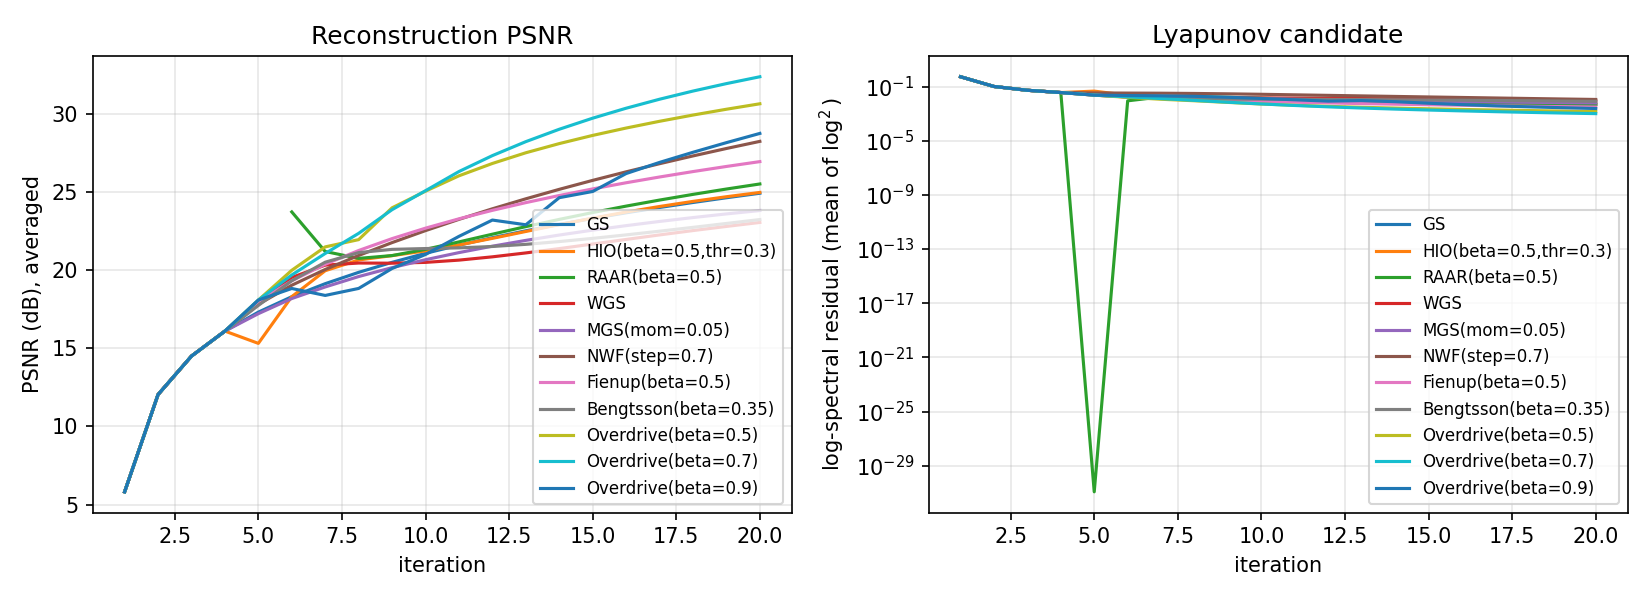
\includegraphics[width=\linewidth]{figures/benchmark.png}
  \caption{(left) PSNR vs.\ iteration, averaged over 29 natural grayscale
  images; (right) log-spectral distance \eqref{eq:lyap}, the Lyapunov
  candidate. Each curve approaches a non-zero plateau --- the kinoform
  synthesis floor of \eqref{eq:ssresid}. The $\beta=0.7$ Overdrive curve has
  the steepest transient slope and the lowest plateau, consistent with the
  prediction that an interior $\beta\in(0,1)$ minimizes both the closed-loop
  pole modulus and the steady-state floor.}
  \label{fig:bench}
\end{figure}

\paragraph{Decay rates.} Figure~\ref{fig:bench} (right panel) shows the
LSD $V_k$ versus iteration. It decays approximately geometrically, consistent
with \eqref{eq:closed_loop}. Geometric-mean per-iteration decay factors over
iterations $5$--$20$ are $0.890$ (GS), $0.872$ (Fienup), $0.929$ (Bengtsson),
$0.829$ ($\beta=0.5$), $\mathbf{0.809}$ ($\beta=0.7$), and $0.857$
($\beta=0.9$). The fastest decay is achieved at the $\beta$ that gives the
highest final PSNR, in agreement with the qualitative prediction
$\beta^{*}\approx c$. The absolute values of the implied $\lvert\beta-c\rvert$
are larger than the linearization \eqref{eq:gs_linearization} predicts; we
attribute this to the noise term $\eta_k$, which is non-negligible for natural
images and dominates the steady-state residual via \eqref{eq:ssresid}. The
linearization is therefore a useful guide to the \emph{ranking} of $\beta$
values rather than a quantitative predictor of absolute decay rate.

\paragraph{Adaptive $\beta$ and the limits of online estimation.} Setting
$\beta^*=c$ requires an estimate of $c$. A natural attempt is to read it off
the LSD trajectory, since $V_k$ decays geometrically with rate $(\beta-c)^2$
during the transient. The released code ({\tt ifta.adaptive}) implements
this and we validate it on synthetic AR(1) trajectories with known
$(\beta,c)$. Two regimes emerge. (i) During the transient, with sufficient
asymmetry between $\beta$ and $c$ (e.g.\ $\beta=0.3$, $c\!\geq\!0.5$), the
estimator recovers $c$ with mean absolute error around $0.2$--$0.3$.
(ii) Near steady state, all such estimators saturate at $V_k/V_{k-1}\!\to\!1$
because $V_k$ does not decay below the floor $V_\infty$; recovering $c$ from
$V_k$ alone is fundamentally impossible once the iteration has converged.
A second, more subtle obstruction is branch ambiguity: $h_k$ depends on
$|\beta-c|$, so $c=\beta\pm|\beta-c|$ are observationally equivalent and
cannot be disambiguated from LSD history alone. For $\beta\!\approx\!0.5$
both branches lie in $[0,1]$ and the estimator must rely on a prior or on
sign information from the unsquared residual, neither of which the LSD
provides. We conclude that online estimation of $c$ is feasible during the
transient phase and useful as a coarse warm-start, but a fixed $\beta$ near
$c$ from offline calibration is more reliable in practice.

% =====================================================================
\section{Discussion}\label{sec:discussion}
% =====================================================================

\paragraph{Relation to other multiplicative IFTA rules.} The Bengtsson rule
\cite{Bengtsson1998}, $\Gkp = \Gkm\,(\F/\Gk)^{\beta}$, lacks the
$\F^{\,2-\beta}/\Gk$ scaling of Overdrive and is therefore not dimensionally
balanced. In log coordinates it becomes $u_k = u_{k-1} - \beta v_k$. Treating
$v_k$ as exogenous, this open-loop response is an accumulator (open-loop pole
at $z=1$); closing the loop through the GS linearization
\eqref{eq:gs_linearization} gives a closed-loop pole at $z = 1-\beta c$, which
is in $(0,1)$ for $\beta,c\in(0,1)$. The rule is therefore stable, not
unstable: Table~\ref{tab:results} confirms it converges. Its empirical
degradation relative to GS on grayscale targets (23.25 vs.\ 24.94~dB) reflects
two effects that the linearization \emph{cannot} compare across rules: a
slower closed-loop pole at typical $\beta\!\ll\!1$, and a different noise
process $\eta_k$ at a different limit cycle. A direct numerical comparison of
the synthesis floors of Bengtsson and Overdrive, controlling for $\eta$, is
left to future work. The Prongu\'e rule \cite{Prongue1992} is the special
case $\beta=1$ of Overdrive and lies on the stability boundary; it works for
sparse point patterns but degrades on grayscale images.

\paragraph{A different problem: phase retrieval.} Wirtinger Flow
\cite{Candes2014} and randomly initialized gradient descent \cite{Chen2018}
provide global convergence guarantees for the non-convex \emph{phase
retrieval} problem, in which a true unknown signal generated the observed
intensity. Their guarantees rely critically on the existence of that true
signal and on assumptions on the measurement matrix (Gaussian, coded
diffraction). They do not transfer to kinoform synthesis, where no
phase-only solution exists in general; what those algorithms would
``recover'' is the closest approximate signal under their loss, which is a
different quantity from the limit cycle of an alternating-projection
scheme. The two literatures should not be conflated.

\paragraph{A different paradigm: deep learning.} Convolutional and
transformer-based phase generators \cite{Zheng2021,Sun2022,Zhu2025} achieve
near-real-time performance by replacing iteration with one trained network
inference. They are class-specific (the network must be trained on a
distribution that resembles the target images) and require dedicated
hardware. They sidestep rather than solve the analytical question studied
here: \emph{how does the synthesis floor of a classical iterative
algorithm depend on its parameters?}.

\paragraph{A different problem statement: Camera-in-the-Loop.} Camera-in-the-Loop
GS \cite{Peng2020} closes the gap between a physical SLM and the idealized
forward model by replacing simulated propagation with measurements from a
camera during training. In a sim-only benchmark such as ours the camera step
is the identity, so CITL reduces to plain GS; including it as a baseline
would be misleading. CITL is the right comparison for hardware deployment
on a specific SLM, not for the parameter-dependence question studied here.
We expect CITL training to compose with Overdrive as a drop-in update rule
on the simulation side; verifying this composition is left to future work.

\paragraph{The role of the dimensional balance.} The exponent $2-\beta$ in
\eqref{eq:overdrive} serves two purposes. First, it ensures that an exact
target $\Gk=\F$ would be a fixed point of the iteration (Section~\ref{sec:rule}),
which is what makes the log-domain residuals $u_k,v_k$ vanish at a hypothetical
zero-residual limit. Second, it produces a closed-loop pole that depends on
$\beta-c$ rather than on the steeper $1-\beta c$ slope of Bengtsson, so that
the optimum $\beta^*=c$ falls in the interior of $(0,1)$ and the noise gain
is unity rather than $\beta$. Whether this translates to a smaller absolute
floor than Bengtsson depends on the (rule-dependent) noise variance, and is
an empirical question --- see Section~\ref{sec:numerics}.

\paragraph{Limitations.} The linearization \eqref{eq:gs_linearization}
captures only the local behaviour of the GS projection at the limit cycle;
far from it, $c$ varies and the analysis is only approximate. The
quantitative agreement of \eqref{eq:ssresid} with the numerical residuals
(Section~\ref{sec:numerics}) is therefore a useful guide to the \emph{ranking}
of $\beta$ values rather than to absolute floor prediction.

% =====================================================================
\section{Conclusion}\label{sec:conclusion}
% =====================================================================

Kinoform synthesis is an approximation problem on the positive orthant of
non-negative amplitudes; its iterative algorithms terminate at a limit
cycle whose distance to the target is the irreducible synthesis floor.
Acceleration with classical Euclidean momentum --- on the phase, on the
gradient of a Wirtinger loss, or on additive correction vectors --- yields
modest gains at best, because the iterate's natural geometry is not
Euclidean. The Overdrive update rule, in retrospect, is Polyak heavy-ball
momentum applied in the negative-entropy mirror geometry, with $\beta$
playing the role of the Polyak momentum coefficient. In log-amplitude
coordinates the rule is a first-order IIR filter with pole at $z=\beta$,
exact by construction; closing the loop through the GS projection moves the
pole to $z=\beta-c$, qualitatively predicting an interior optimum at
$\beta\approx c$. The L\textsuperscript{2} hologram-plane error is not the
right Lyapunov function for this rule --- the log-spectral distance (the
Bregman divergence of the mirror map) is. The AR(1)-with-white-noise
closed-loop model that would give a closed-form synthesis floor is
empirically refuted by an autocorrelation test on the innovations; the
linearization is informative for ranking $\beta$ values but not as a
quantitative floor predictor. On 29 natural grayscale images, Overdrive at
$\beta=0.7$ reaches a mean PSNR of $32.4$~dB after twenty iterations,
exceeding plain GS by $7.5$~dB, all three alternating-projection baselines
(HIO, RAAR, WGS) by at least $6.9$~dB, and Nesterov-accelerated Wirtinger
Flow --- the natural additive-momentum competitor --- by $4.1$~dB.

\paragraph{Code and data availability.} A reference Python implementation of
all algorithms discussed, together with the benchmark scripts and image set
used in Table~\ref{tab:results}, is available at
\url{https://github.com/Sneakerx/ifta}.

\bibliography{overdrive_stability}

\end{document}
